\newcommand{\Title}{Robadge\#1} 
\title{\Title}

\documentclass[a4paper]{article}
\usepackage{geometry}
\geometry{a4paper,tmargin=25mm,bmargin=35mm,lmargin=20mm,rmargin=20mm,footskip=5mm}
\usepackage[utf8x]{inputenc}
\usepackage{fontspec}
\usepackage{graphicx}
\usepackage{subcaption}
\usepackage{capt-of}
\usepackage{multirow} 
\usepackage[ngerman]{babel}
\usepackage[colorlinks=true,linkcolor=black,urlcolor=black]{hyperref}
\usepackage[headsepline,footsepline]{scrlayer-scrpage}


\usepackage{xcolor,soul}
\usepackage{colortbl} % Farbige Tabellen

\usepackage{longtable}

\pagestyle{scrheadings}
\clearscrheadfoot

\definecolor{LightGray}{rgb}{0.9,0.9,0.9}
\newcommand{\CItoprowcolor}{\rowcolor{LightGray}}

%%Head
\ihead{{\textbf{\large \Title}}}
\ohead{\raisebox{0.1\totalheight}{
\includegraphics[width=0.15\textwidth]{../pictures/wak-lab-LOGO.png}}}

%%Foot
\cfoot{\pagemark}
\ofoot{\today}

\addto\captionsngerman{
\renewcommand{\figurename}{Abb.}
\renewcommand{\tablename}{Tab.}
}

\newcommand\Vorsicht[1]{%
%\setlength\arrayrulewidth{1,50pt}
\ \\
\begin{tabular}{p{0.16\textwidth} p{0.79\textwidth}|}
\cline{2-2}
& \\
 \multirow{5}{*}{\raisebox{0mm}[0mm][0mm]{
\includegraphics[width=0.1\textwidth]{../pictures/Vorsicht.png}}} & \textbf{VORSICHT!}{\begin{flushleft}#1\end{flushleft}} \\
\cline{2-2}
\end{tabular}
\ \\
%\setlength\arrayrulewidth{0,75pt}
}


\begin{document}
\maketitle
%\tableofcontents
\begin{center}
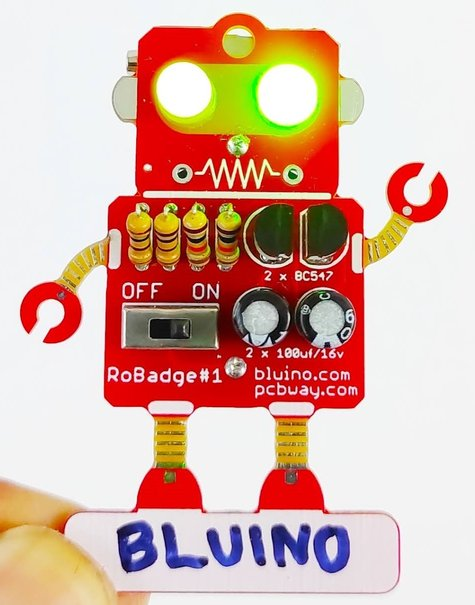
\includegraphics[height=8cm]{../pictures/Ready.jpg}\ \\
\ \\

\includegraphics[height=1cm]{../pictures/header-bluino.png}
\ \\
\ \\
By Bluino \\
September 21, 2020 \\
\end{center}
\newpage
\section{Einleitung}
Der Bausatz ist gedacht als Lötübung für eine Blinkschaltung (Flip-Flop) mit zwei LEDs, zwei Transistoren, zwei Kondensatoren, vier Widerständen, ein Schalter und einer Knopfzelle CR2032.\\
Im Schaltplan sieht man, dass die Spannung vom Minuspol der Batterie (3V) erst durch die Schalter muss. Wenn dieser eingeschaltet ist, kann der Strom in der Schaltung fließen.\\
\ \\
\begin{minipage}[t]{\textwidth}
  \centering
  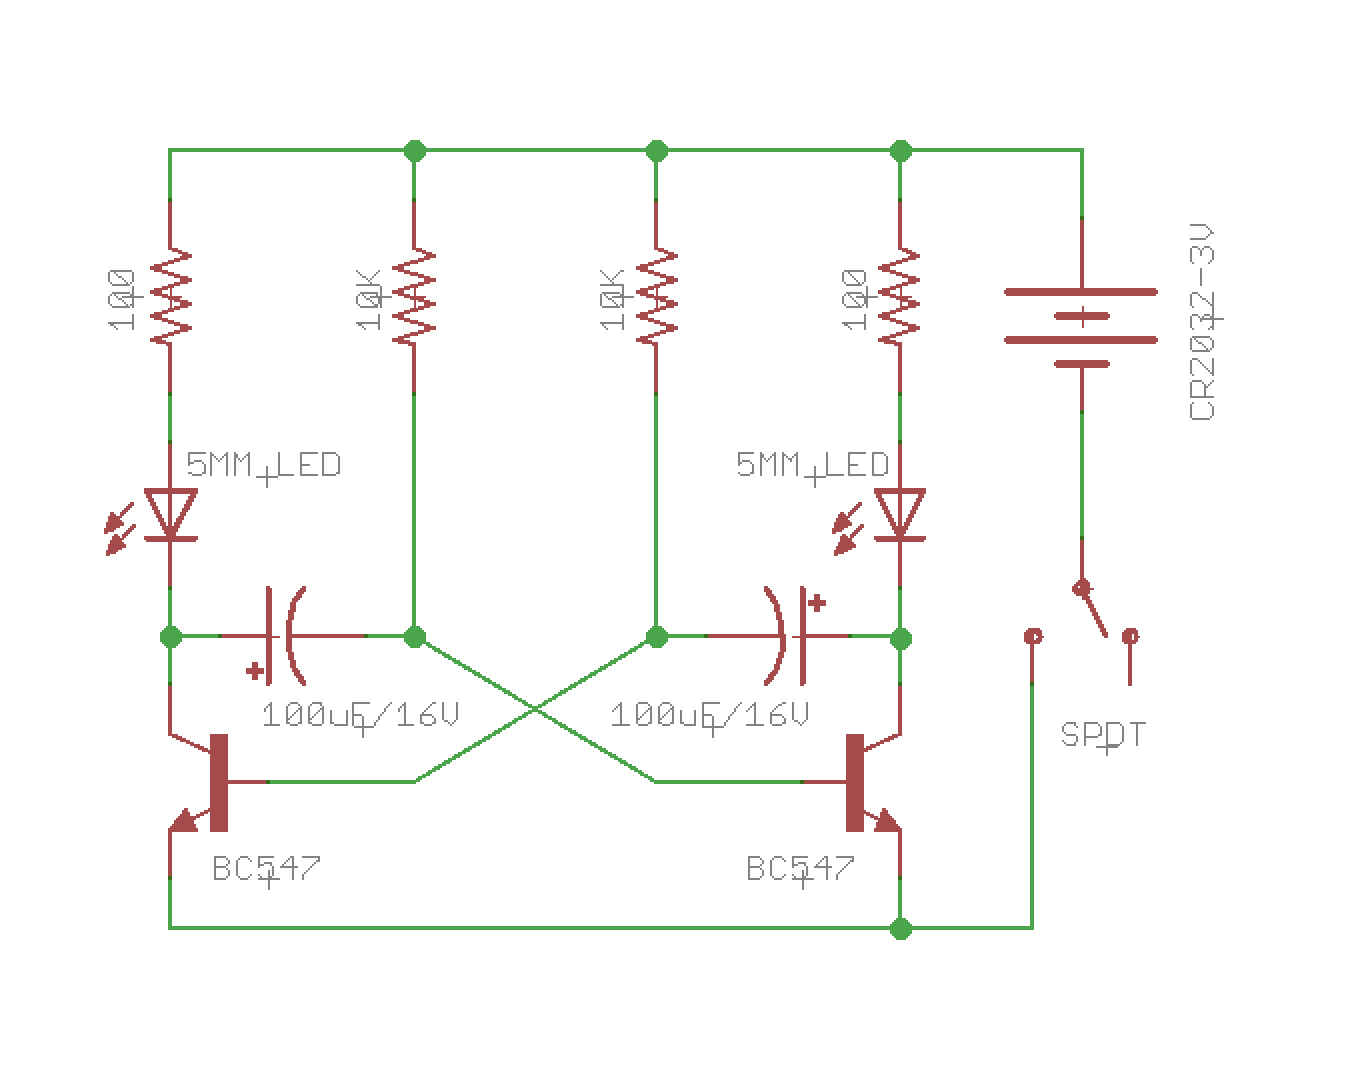
\includegraphics[width=0.55\textwidth]{../pictures/schematic.png}
  \captionof{figure}{Schaltplan}
  \label{img:Schematic}
\end{minipage}
\ \\
\Vorsicht{\begin{itemize} \item der Lötkolben ist sehr \textbf{heiß}. Niemals mit den Fingern berühren!
\item die Lötdämpfe \textbf{nicht} einatmen \item nach der Arbeit bitte die Hände mit Seife waschen\item beim Abschneiden der Beinchen bitte darauf achten, dass Sie nicht durch die Luft fliegen\end{itemize}}\\
\ \\
\newpage

\section{Aufbau}
\begin{minipage}[t]{\textwidth}
  \centering
  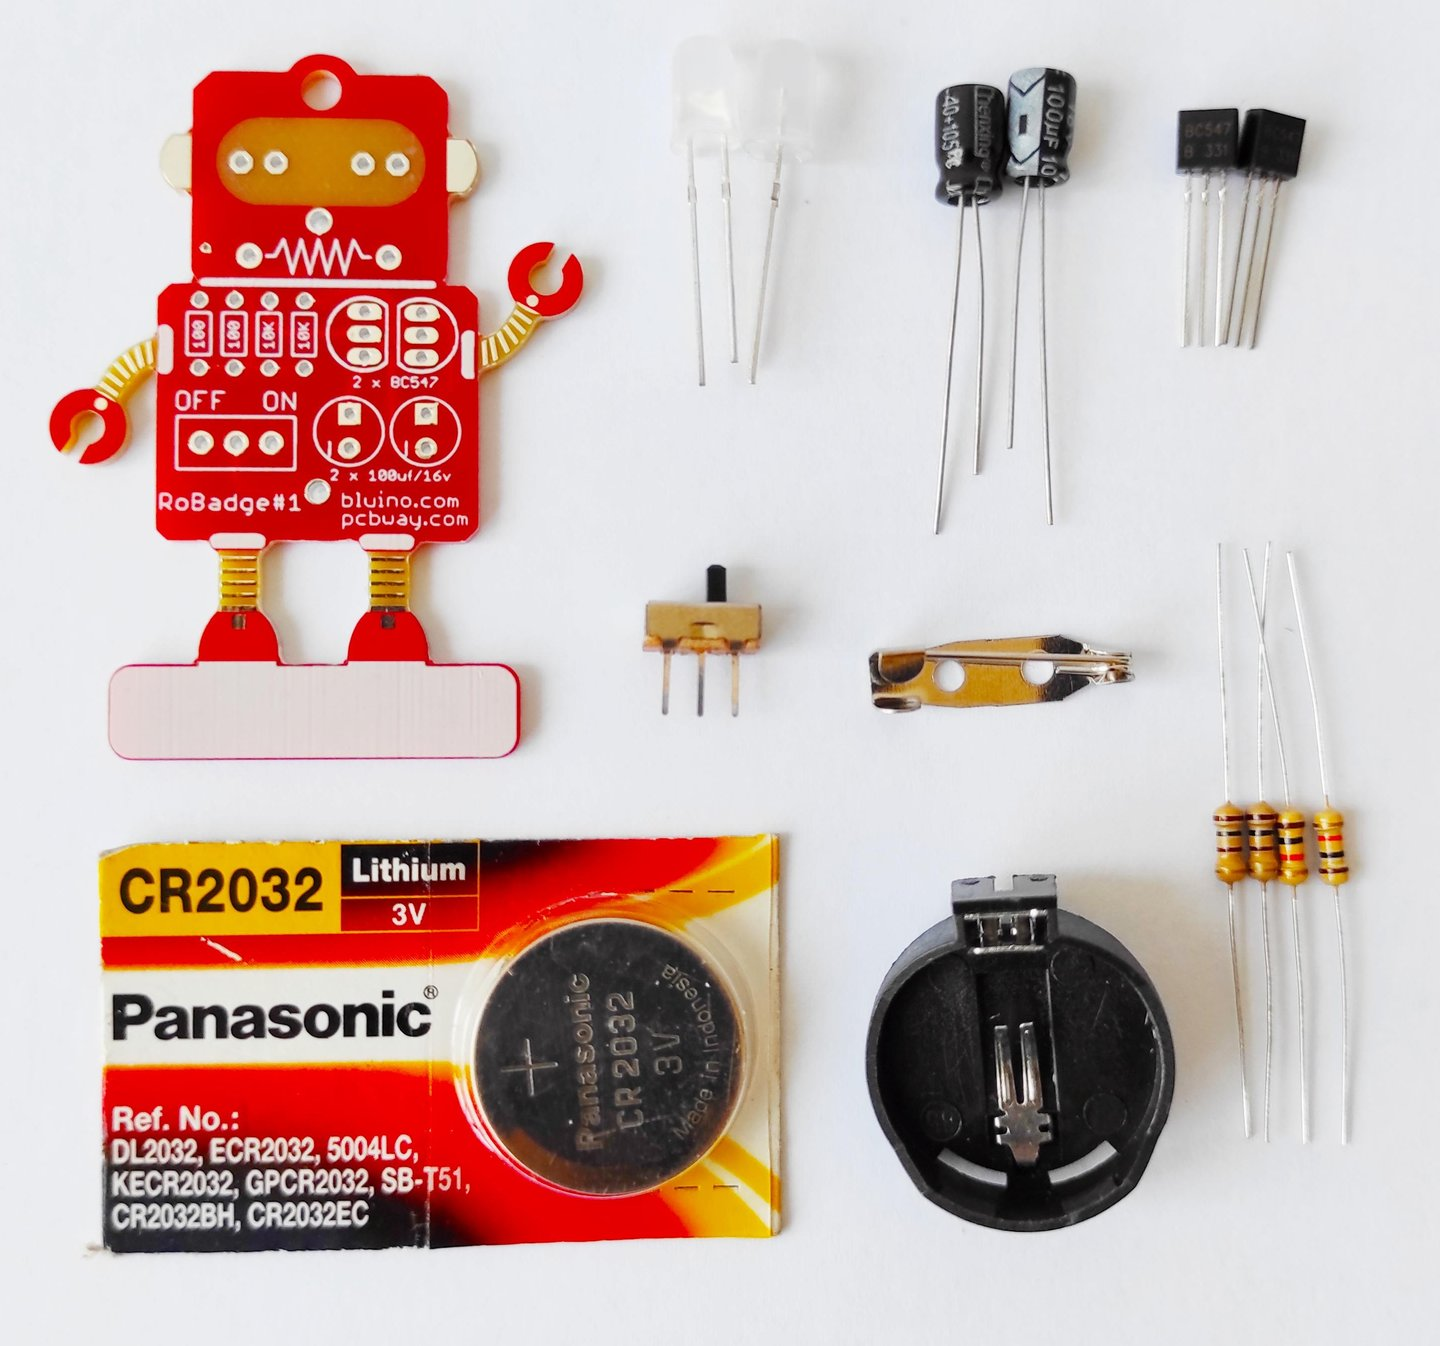
\includegraphics[width=0.9\textwidth]{../pictures/Partlist.jpg}
  \captionof{figure}{Bauteile}
  \label{img:Bauteile}
\end{minipage}
\ \\
Bauteile:
\begin{itemize}
  \item     1x PCB Robadge\#1
  \item     2x Transistor NPN BC527
  \item     2x LED 5mm
  \item     2x C 100uF/16V
  \item     2x R 100 ohm 1/4W
  \item     2x R 10K ohm 1/4W
  \item     1x Switch 3pin SPDT SS12D00G3
  \item     1x Knopfzelle CR2032
  \item     1x Batteriehalter THT CR2032
  \item     1x Anstecknadel, 25mm 
\end{itemize}
\subsection{Schritt 1 - Bauteile einsetzen}
\begin{minipage}[t]{0.28\textwidth}
  \centering
  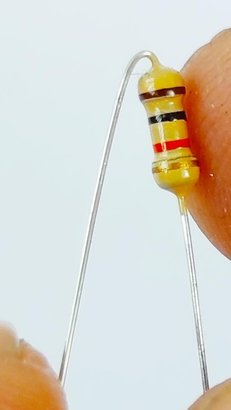
\includegraphics[height=4.5cm]{../pictures/Resistor1.jpg}
  \captionof{figure}{Widerstände knicken}
  \label{img:Resistor1}
  \end{minipage}
\begin{minipage}[t]{0.30\textwidth}
  \centering
  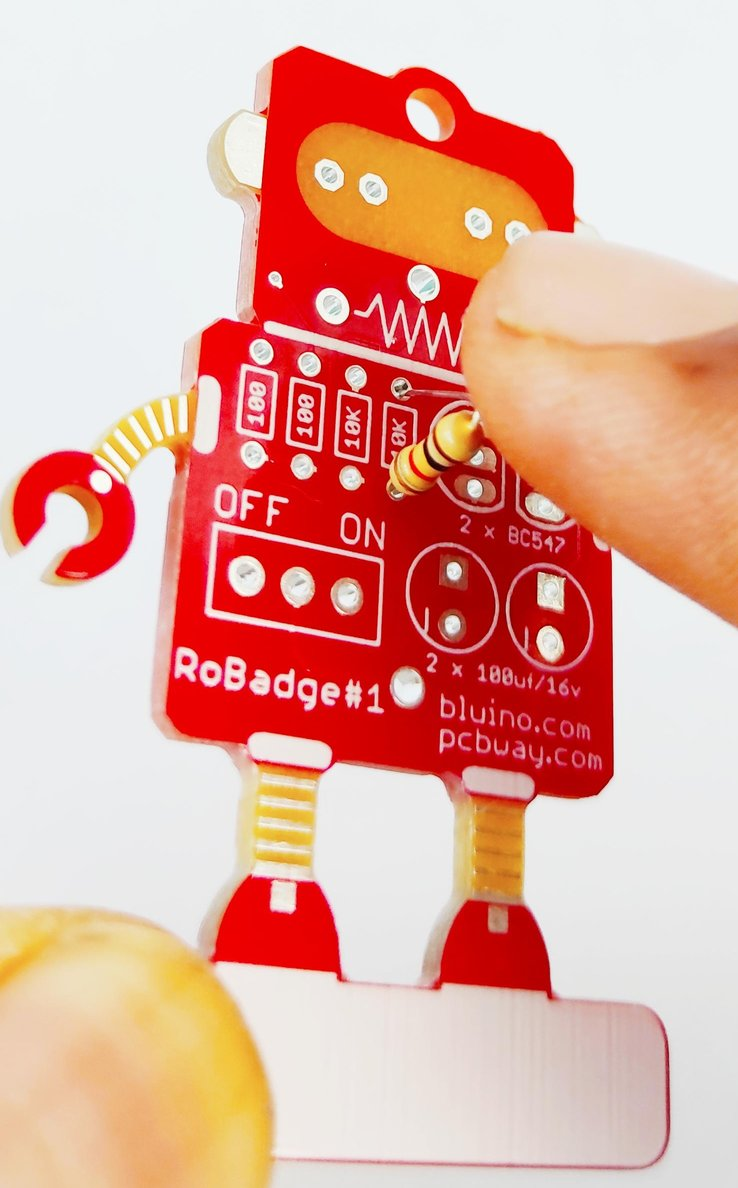
\includegraphics[height=4.5cm]{../pictures/Resistor2.jpg}
  \captionof{figure}{Widerstände einfädeln}
  \label{img:Resistor2}
\end{minipage}
\begin{minipage}[t]{0.40\textwidth}
  \centering
  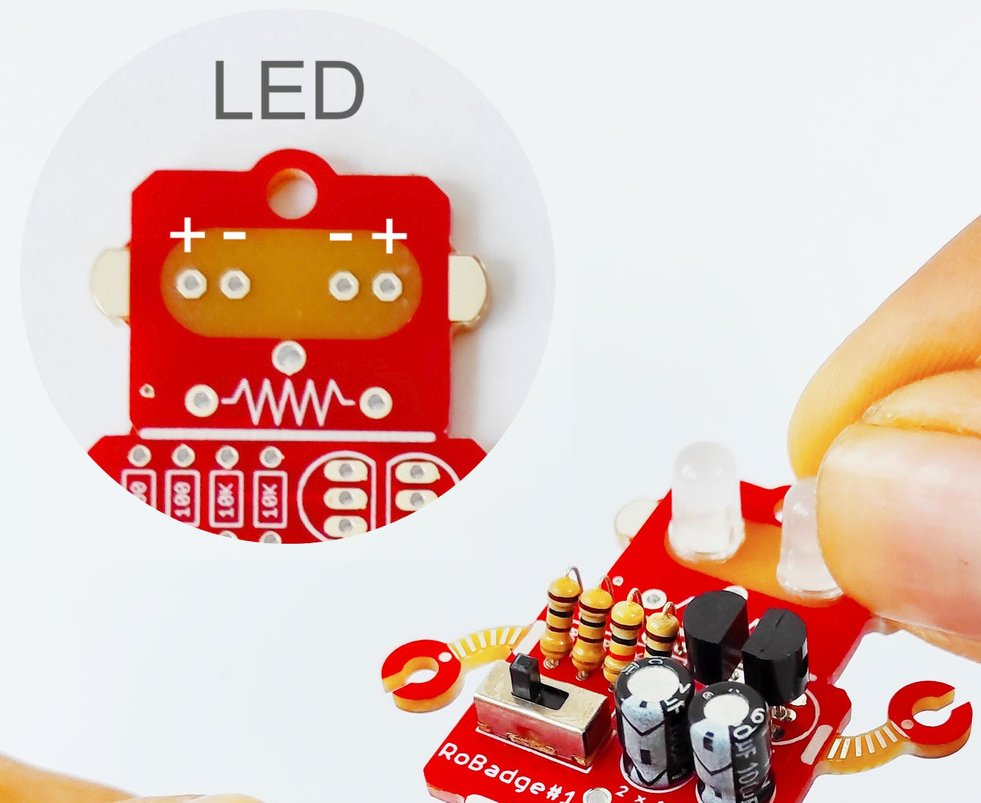
\includegraphics[height=4.5cm]{../pictures/LED1.jpg}
  \captionof{figure}{Bauteile einsetzen}
  \label{img:Resistor3}
\end{minipage}
\ \\
\begin{itemize}
\item das lange LED-Beinchen bei + einfädeln
\item das lange Kondensator-Beinchen nach oben
\item links zwei Widerstände mit Braun-Schwarz-Braun-Gold (100 Ohm)
\item mittig zwei Widerstände mit Braun-Schwarz-Rot-Gold (10 kOhm)
\item die Transistoren schauen sich gegenseitig an
\end{itemize}

\begin{minipage}[t]{\textwidth}
  \centering
  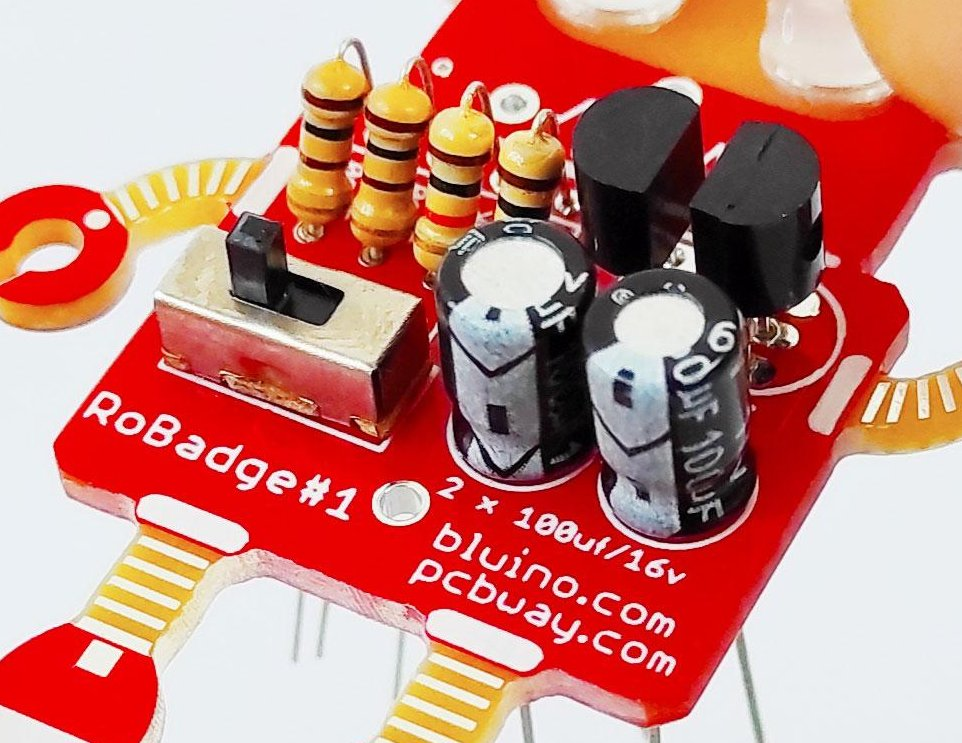
\includegraphics[width=0.33\textwidth]{../pictures/Bestueckung.jpg}
  \captionof{figure}{Bestueckung}
  \label{img:Bestueckung}
\end{minipage}
\subsection{Schritt 2 - Bauteile verlöten}
\begin{minipage}[t]{0.28\textwidth}
  \centering
  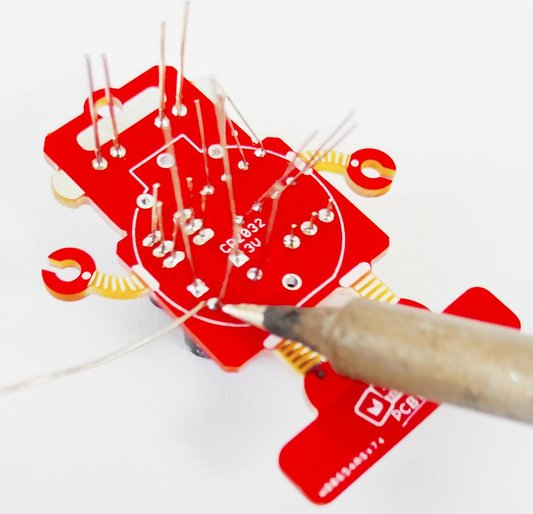
\includegraphics[height=4.5cm]{../pictures/Loeten.jpg}
  \captionof{figure}{Löten}
  \label{img:Loeten}
  \end{minipage}
\begin{minipage}[t]{0.33\textwidth}
  \centering
  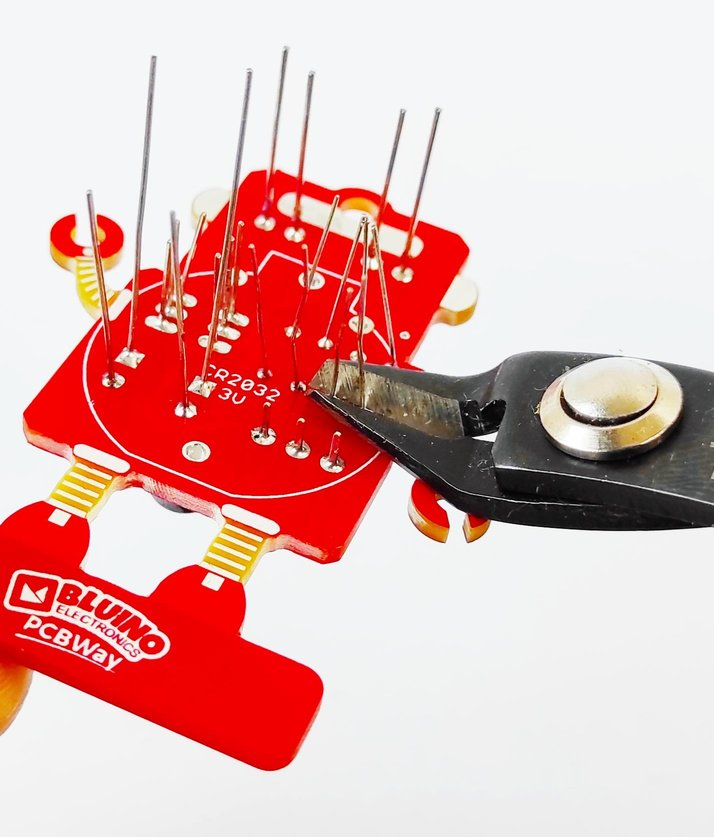
\includegraphics[height=4.5cm]{../pictures/Cut.jpg}
  \captionof{figure}{Beinchen abschneiden}
  \label{img:Cut}
\end{minipage}
%\begin{minipage}[t]{0.33\textwidth}
%  \centering
%  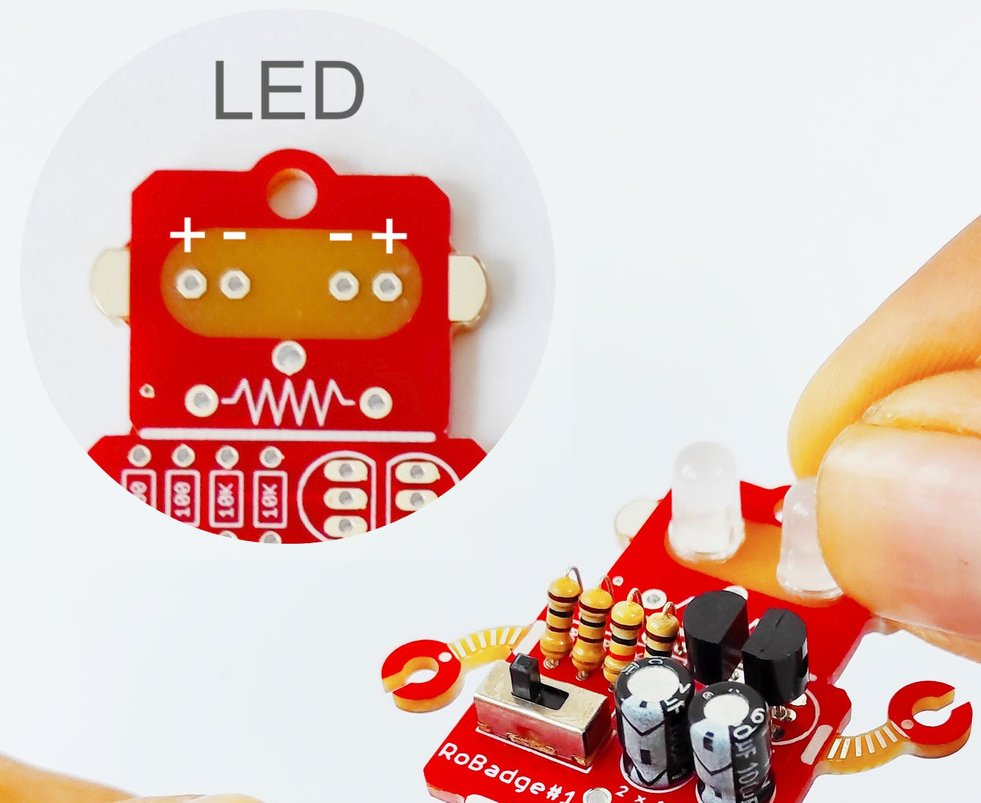
\includegraphics[height=4.5cm]{../pictures/LED1.jpg}
%  \captionof{figure}{Bauteile Einsetzen}
%  \label{img:Resistor3}
%\end{minipage}
\ \\
\subsection{Schritt 3 - Batteriehalter und Anstecknadel}
\begin{minipage}[t]{0.33\textwidth}
  \centering
  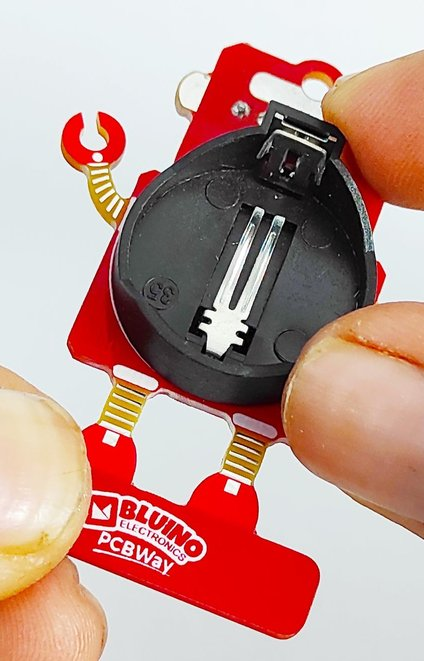
\includegraphics[height=4.5cm]{../pictures/Battery.jpg}
  \captionof{figure}{Halter einstecken}
  \label{img:Halter}
  \end{minipage}
\begin{minipage}[t]{0.33\textwidth}
  \centering
  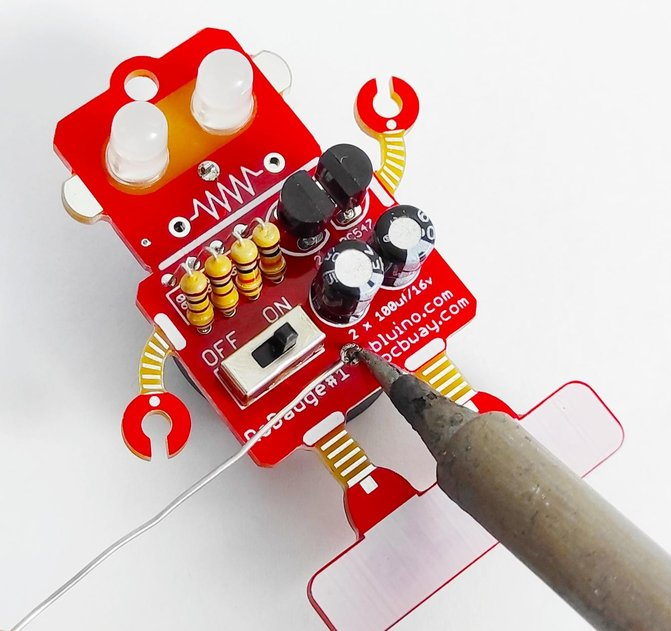
\includegraphics[height=4.5cm]{../pictures/Loeten2.jpg}
  \captionof{figure}{Halter anlöten}
  \label{img:Loeten2}
\end{minipage}
\begin{minipage}[t]{0.33\textwidth}
  \centering
  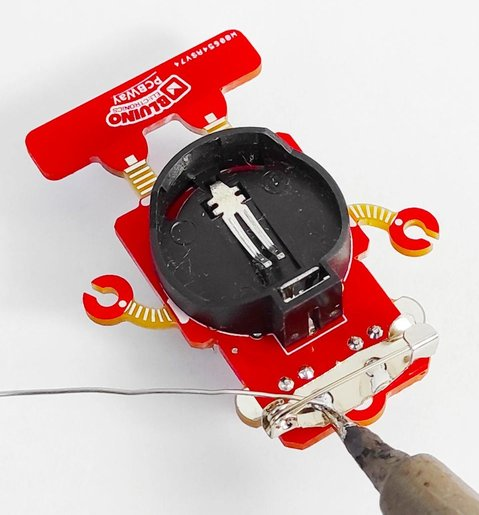
\includegraphics[height=4.5cm]{../pictures/Halter.jpg}
  \captionof{figure}{Anstecknadel anlöten}
  \label{img:Loeten2}
\end{minipage}
\subsection{Schritt 4 - fertigstellen}
\begin{minipage}[t]{0.33\textwidth}
  \centering
  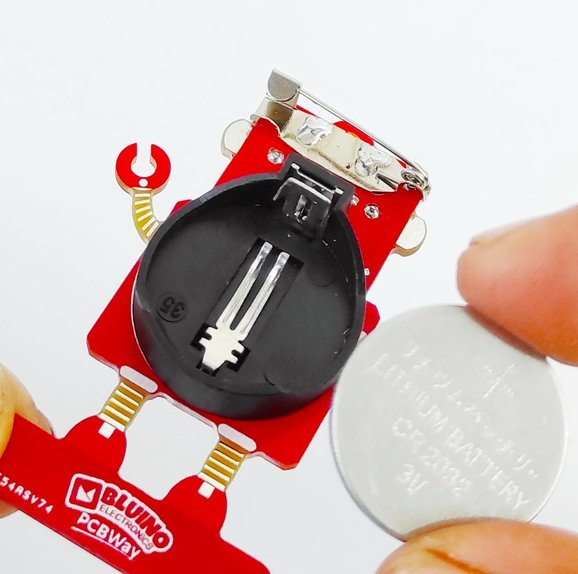
\includegraphics[height=4.5cm]{../pictures/Knopfzelle.jpg}
  \captionof{figure}{Knopfzelle einsetzen}
  \label{img:Knopfzelle}
  \end{minipage}
\begin{minipage}[t]{0.33\textwidth}
  \centering
  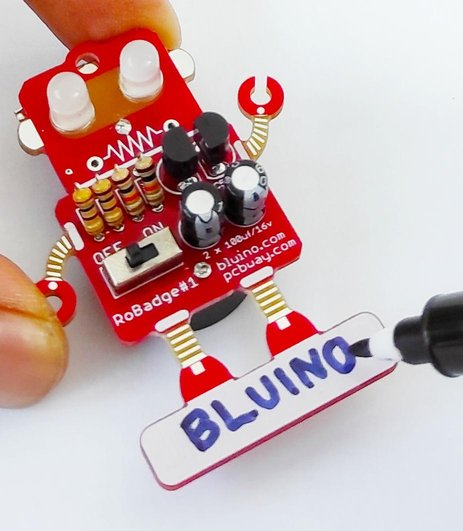
\includegraphics[height=4.5cm]{../pictures/Name.jpg}
  \captionof{figure}{Name schreiben}
  \label{img:Name}
\end{minipage}
\begin{minipage}[t]{0.33\textwidth}
  \centering
  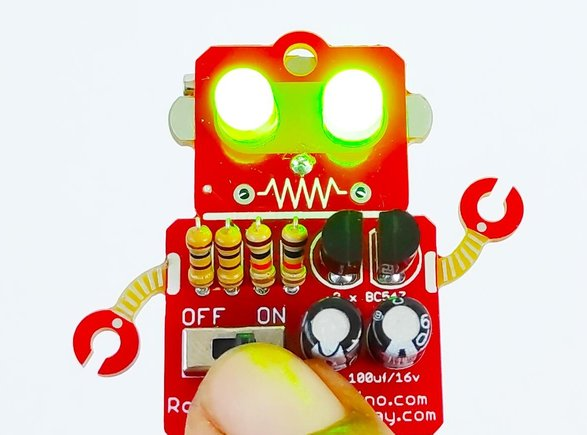
\includegraphics[height=4.5cm]{../pictures/Switchon.jpg}
  \captionof{figure}{einschalten}
  \label{img:Switchon}
\end{minipage}
\ \\
\end{document}

